%\documentclass[a4paper,english,11pt,twoside]{article}
\documentclass[a4paper,english,11pt]{article}

\usepackage[utf8]{inputenc}
\usepackage[T1]{fontenc, url}
\usepackage[english]{babel}
%\usepackage{epsfig}
\usepackage{graphicx}
\usepackage{amsmath}
\usepackage{mathtools}
\usepackage{pstricks}
\usepackage{subfig}
\usepackage{epstopdf}
\usepackage{varioref}
\usepackage{listings}
\usepackage{xcolor}
\usepackage{float}
\usepackage[]{mcode}
\usepackage{verbatim}
\lstset{ 
  captionpos=b,
  frame=tb,
  numbers=left}
\urlstyle{sf}
\usepackage[margin=1 in]{geometry} % Setter margene til word standard

\usepackage{ifikompendiumforside}


\newcommand{\tab}[1]{\hspace{.2\textwidth}\rlap{#1}}

\newcommand{\itab}[1]{\hspace{0em}\rlap{#1}}

%%%%%%%%%%%%%%%%%% END HEADER

\title{Laboratory Assignment 3}
\subtitle{INF4411\\ 
          Analog Microelectronics}

\author{
\begin{tabular}{ r c l }
  Rikesh Chauhan & & rikesh.chauhan@fys.uio.no\\
  Espen Klein Nilsen & & e.a.k.nilsen@fys.uio.no\\
  Vegard Midtbøen & & vegard.midtboen@fys.uio.no
\end{tabular}
}
%{Rikesh Chauhan rikesh.chauhan@fys.uio.no\\
%	Espen Klein Nilsen e.a.k.nilsen@fys.uio.no\\
%	Vegard Midtbøen vegard.midtboen@fys.uio.no} 

\begin{document}
\ififorside

\tableofcontents

\newpage
%//////////////////////////////////////Task1///////////////////////////////////////////////////////////////////////        
\section{Task 1}
The circuit shown in Figure \ref{fig:chem} shows the chematic drawn in Cadence for the given curcuit.
\begin{figure}[!htbp]
 \centering
  \fbox{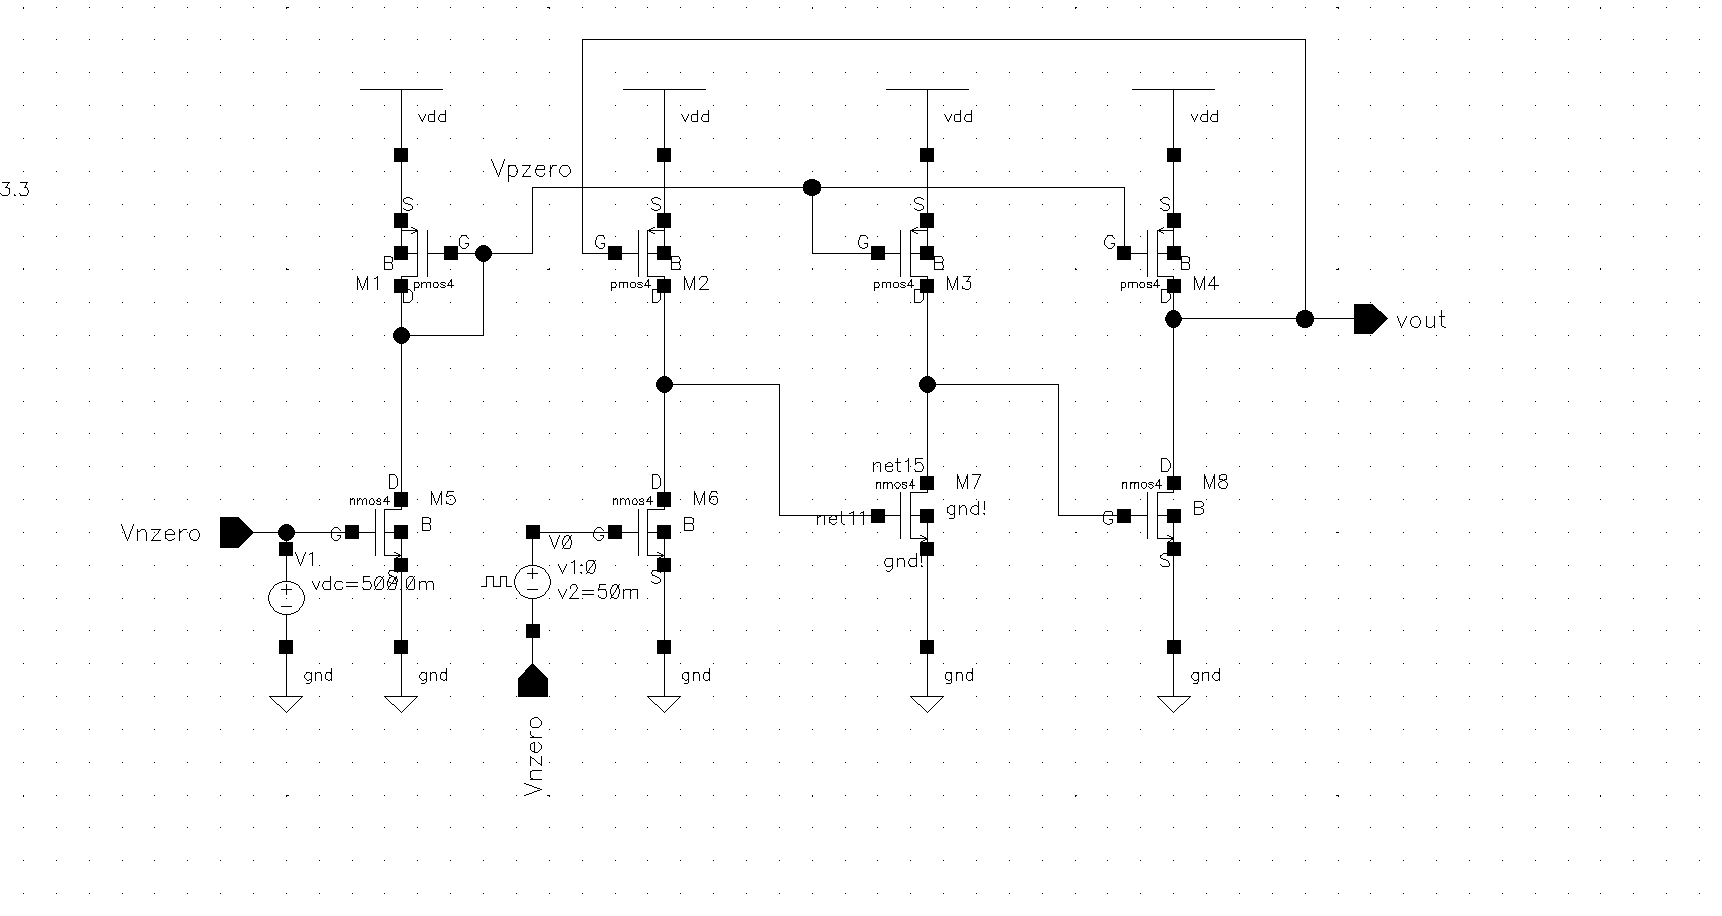
\includegraphics[width=\textwidth]{img/chematic_bi-color}}
  \caption{Chematic drawing from Cadence.}
  \label{fig:chem}	
\end{figure}


\section{Task 2}
\textbf{1.1}\\
The simulation parameters we used for this simulation is listed below:\\
\begin{enumerate}
  \item \itab{$V_{DD}$:} \tab{3.3 V}
  \item \itab{$V_{nzero}$:} \tab{500 mV} \tab{(DC-Offset)}
  \item \itab{$V_{step}$:} 
  \begin{enumerate}
    \item \itab{$Amplitude$:} \tab{$50 mV$}
    \item \itab{$Rise time$:} \tab{$100 ns$}
  \end{enumerate}
  \item \itab{W/L} \tab{$10\mu m/0.35\mu m$}  
  \item \itab{$V_{sweep}$} \tab{0 - 6 V}
\end{enumerate}
A plot of the output and input for the circuit is shown in Figure \ref{fig:sim:ring}. From the plot we can se that 
after a \textit{steep} step we get oscillations on the output that reaches $Vdd$. The peak to peak voltage is $1.2 V$.
The simulation is so resource intencive that we were forced to only run the simulation for a short time (or shorter 
than the task spesified).\\



\begin{figure}[!htbp]
 \centering
  \fbox{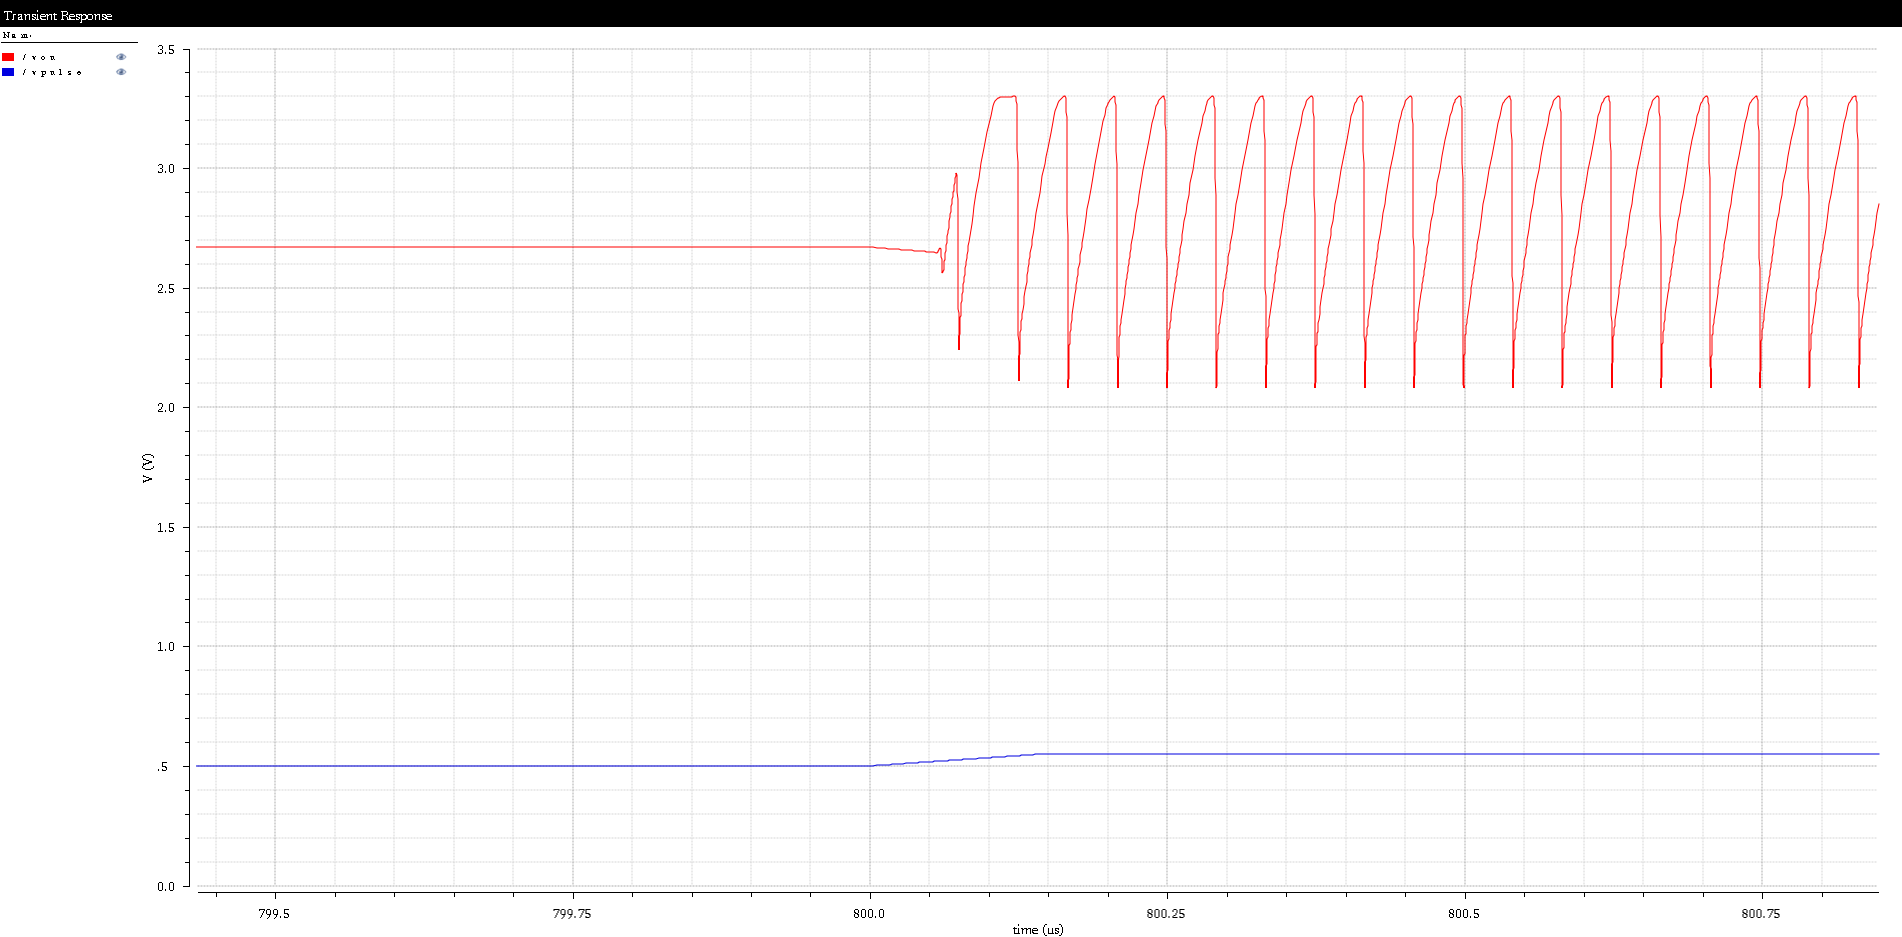
\includegraphics[width=\textwidth]{img/simulation_with_ringing}}
  \caption{Simulation with ringing.}
  \label{fig:sim:ring}	
\end{figure}
\newpage
\textbf{1.2}\\
The AC responce is plottet in Figure \ref{fig:ac:responce}\\
\begin{figure}[!htbp]
 \centering
  \fbox{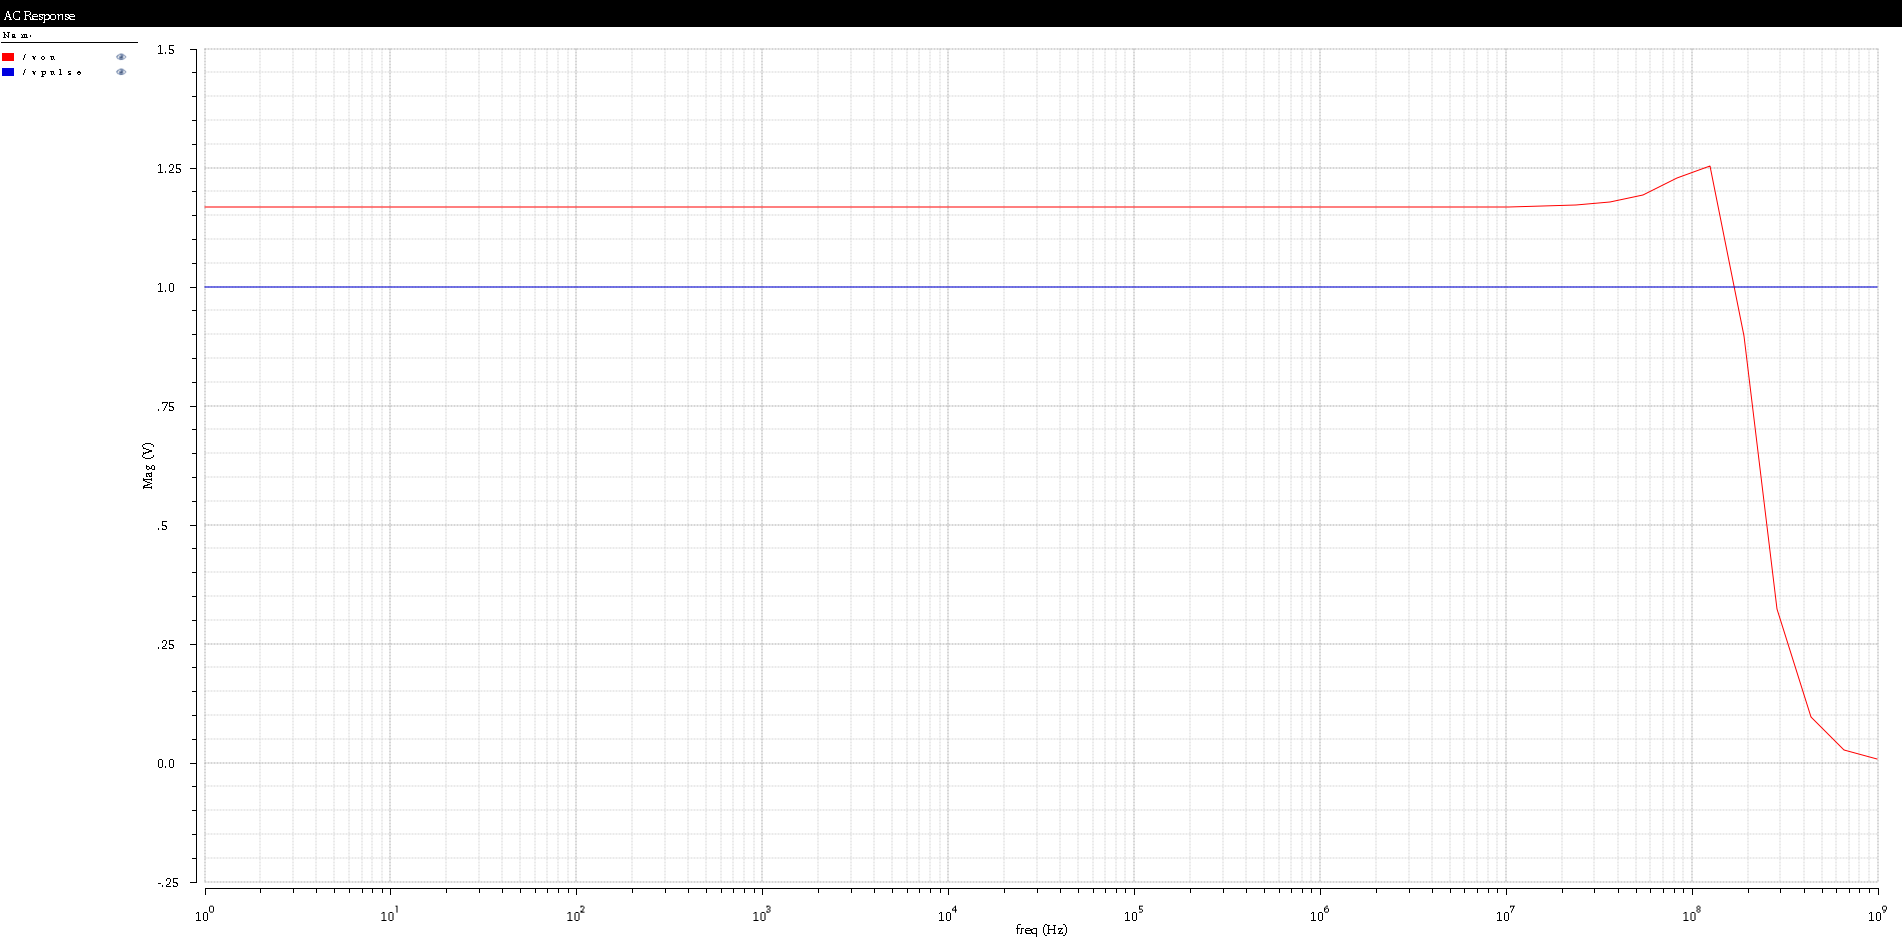
\includegraphics[width=\textwidth]{img/ac_responce}}
  \caption{Plot of AC responce.}
  \label{fig:ac:responce}	
\end{figure}

The frequency of the oscillations is about 24 MHz in the cadence simulation. There is a maximum at 120MHz in the AC-simulation. The   resonance appears to start at 24MHz, witch could give rise to the ringing on the output. 

\section{Task 3}

\section{Task 4}

\section{Task 5}
Figure \ref{fig:pcb} shows the PCB for this task. We decided to make a new PCB because the awailable transistor in the lab, was not the same as in the previos labs.
\begin{figure}[!htbp]
 \centering
  \fbox{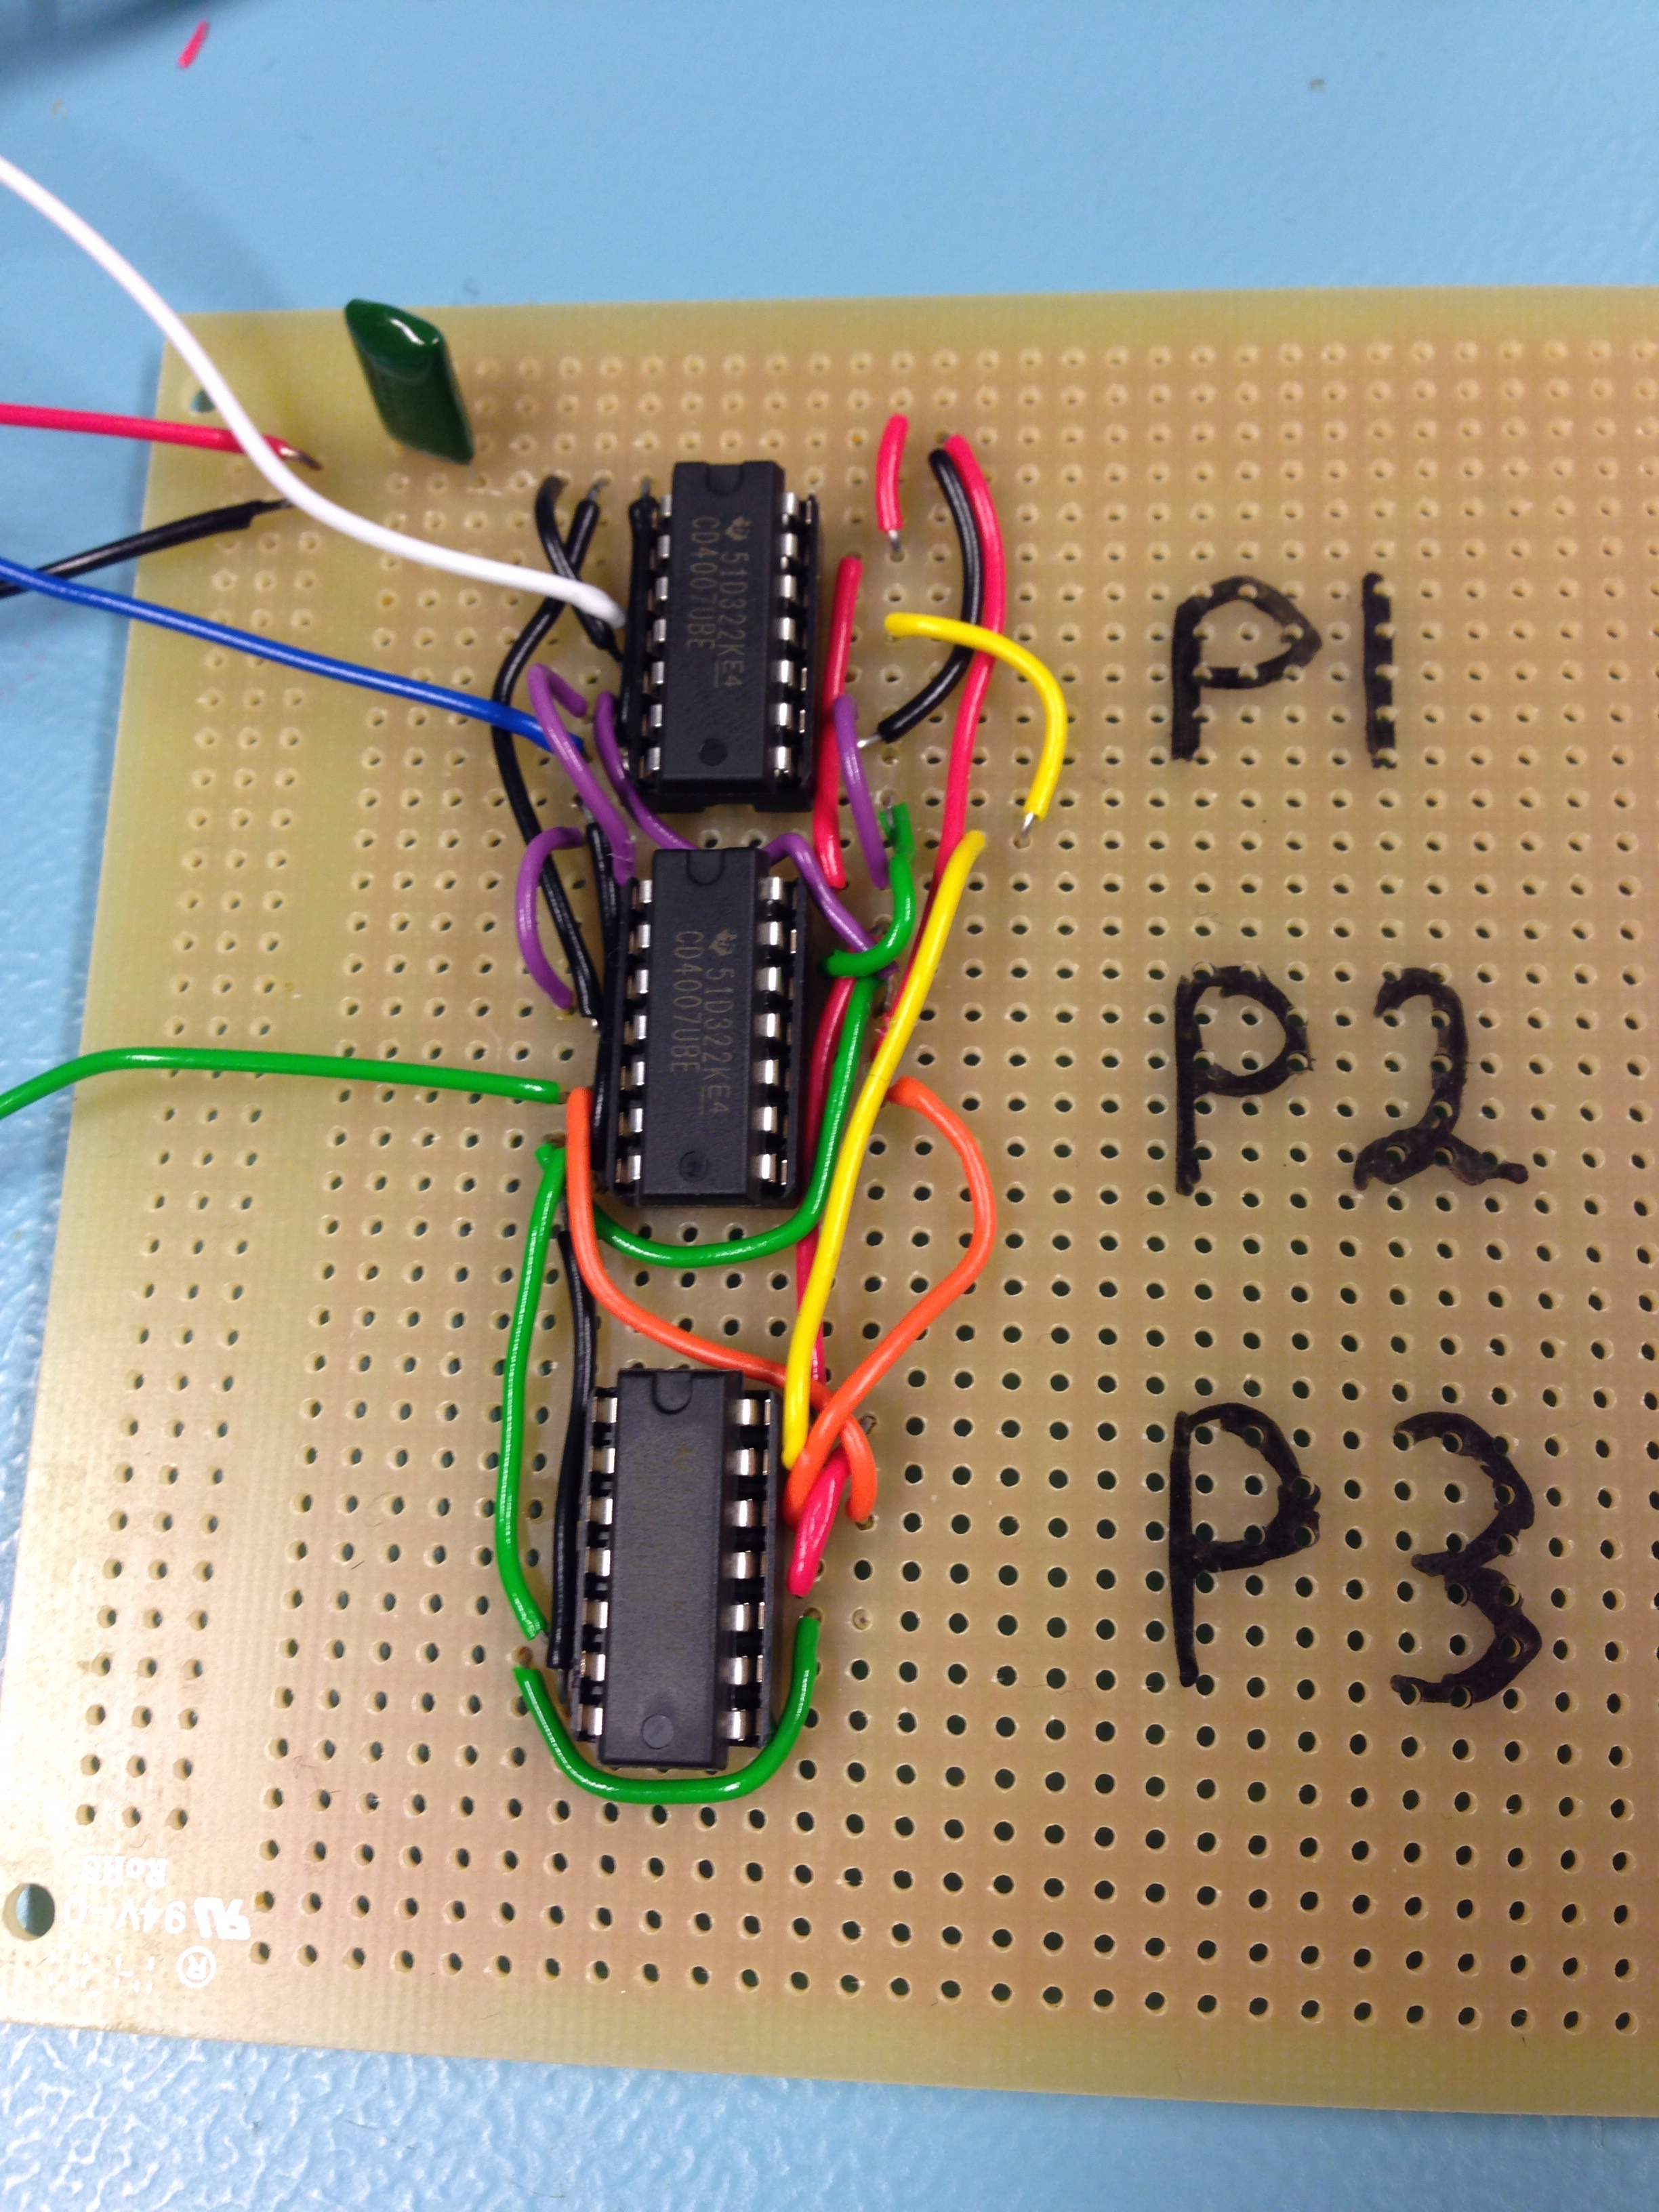
\includegraphics[width=0.8\textwidth]{img/pcb}}
  \caption{PCB for task 5.}
  \label{fig:pcb}	
\end{figure}
In the task, it was given that $V_{DD}$ was suppose to be $10 V$. For $V_{DD}$ we used the voltage source available in the lab, and used the $+ 25V$ port.
The voltage for $V_{nzero}$ was also provided from the voltage source, using the $+ 6V$ port.\\
\\
To find a proper $V_{nzero}$, we connencted the oscilloscope to the output. By doing this, we could determine which value for $V_{nzero}$ that gave the 
most symetrical outout. We found this bias voltage to be $3.8V$. When this was set, we made a simple matlab script (see appendix X), controlling the 
voltage supply and the oscilloscope. The plot for the output can be seen in Figure \ref{fig:oscil:out}.\\
\\
The circuit is not stable. What we see from the plot in Figure \ref{fig:oscil:out} is oscillation/ringing. The frequency for the oscillation is
$5.348 MHz$.
\begin{figure}[!htbp]
 \centering
  \fbox{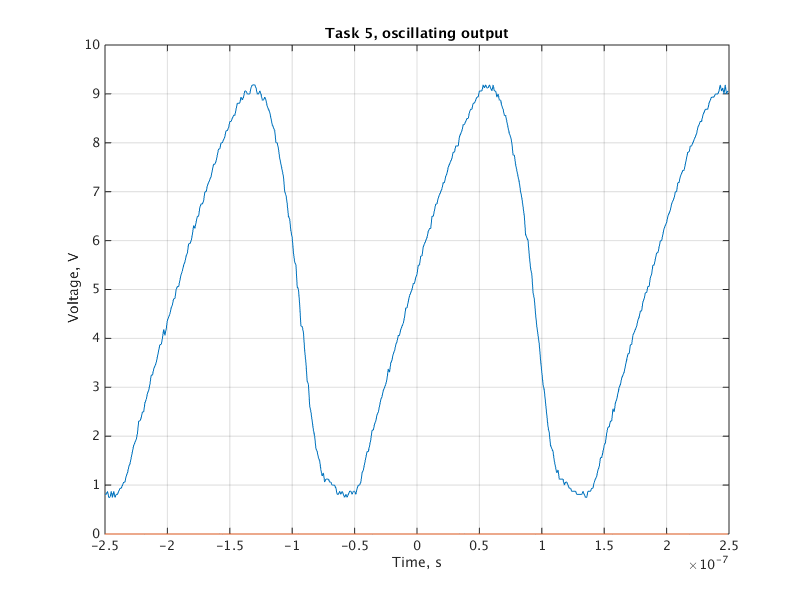
\includegraphics[width=\textwidth]{img/task5_oscillating_output}}
  \caption{Oscillating output at Vdd/2.}
  \label{fig:oscil:out}	
\end{figure}

%\begin{figure}[htbp]
% \centering
%  \fbox{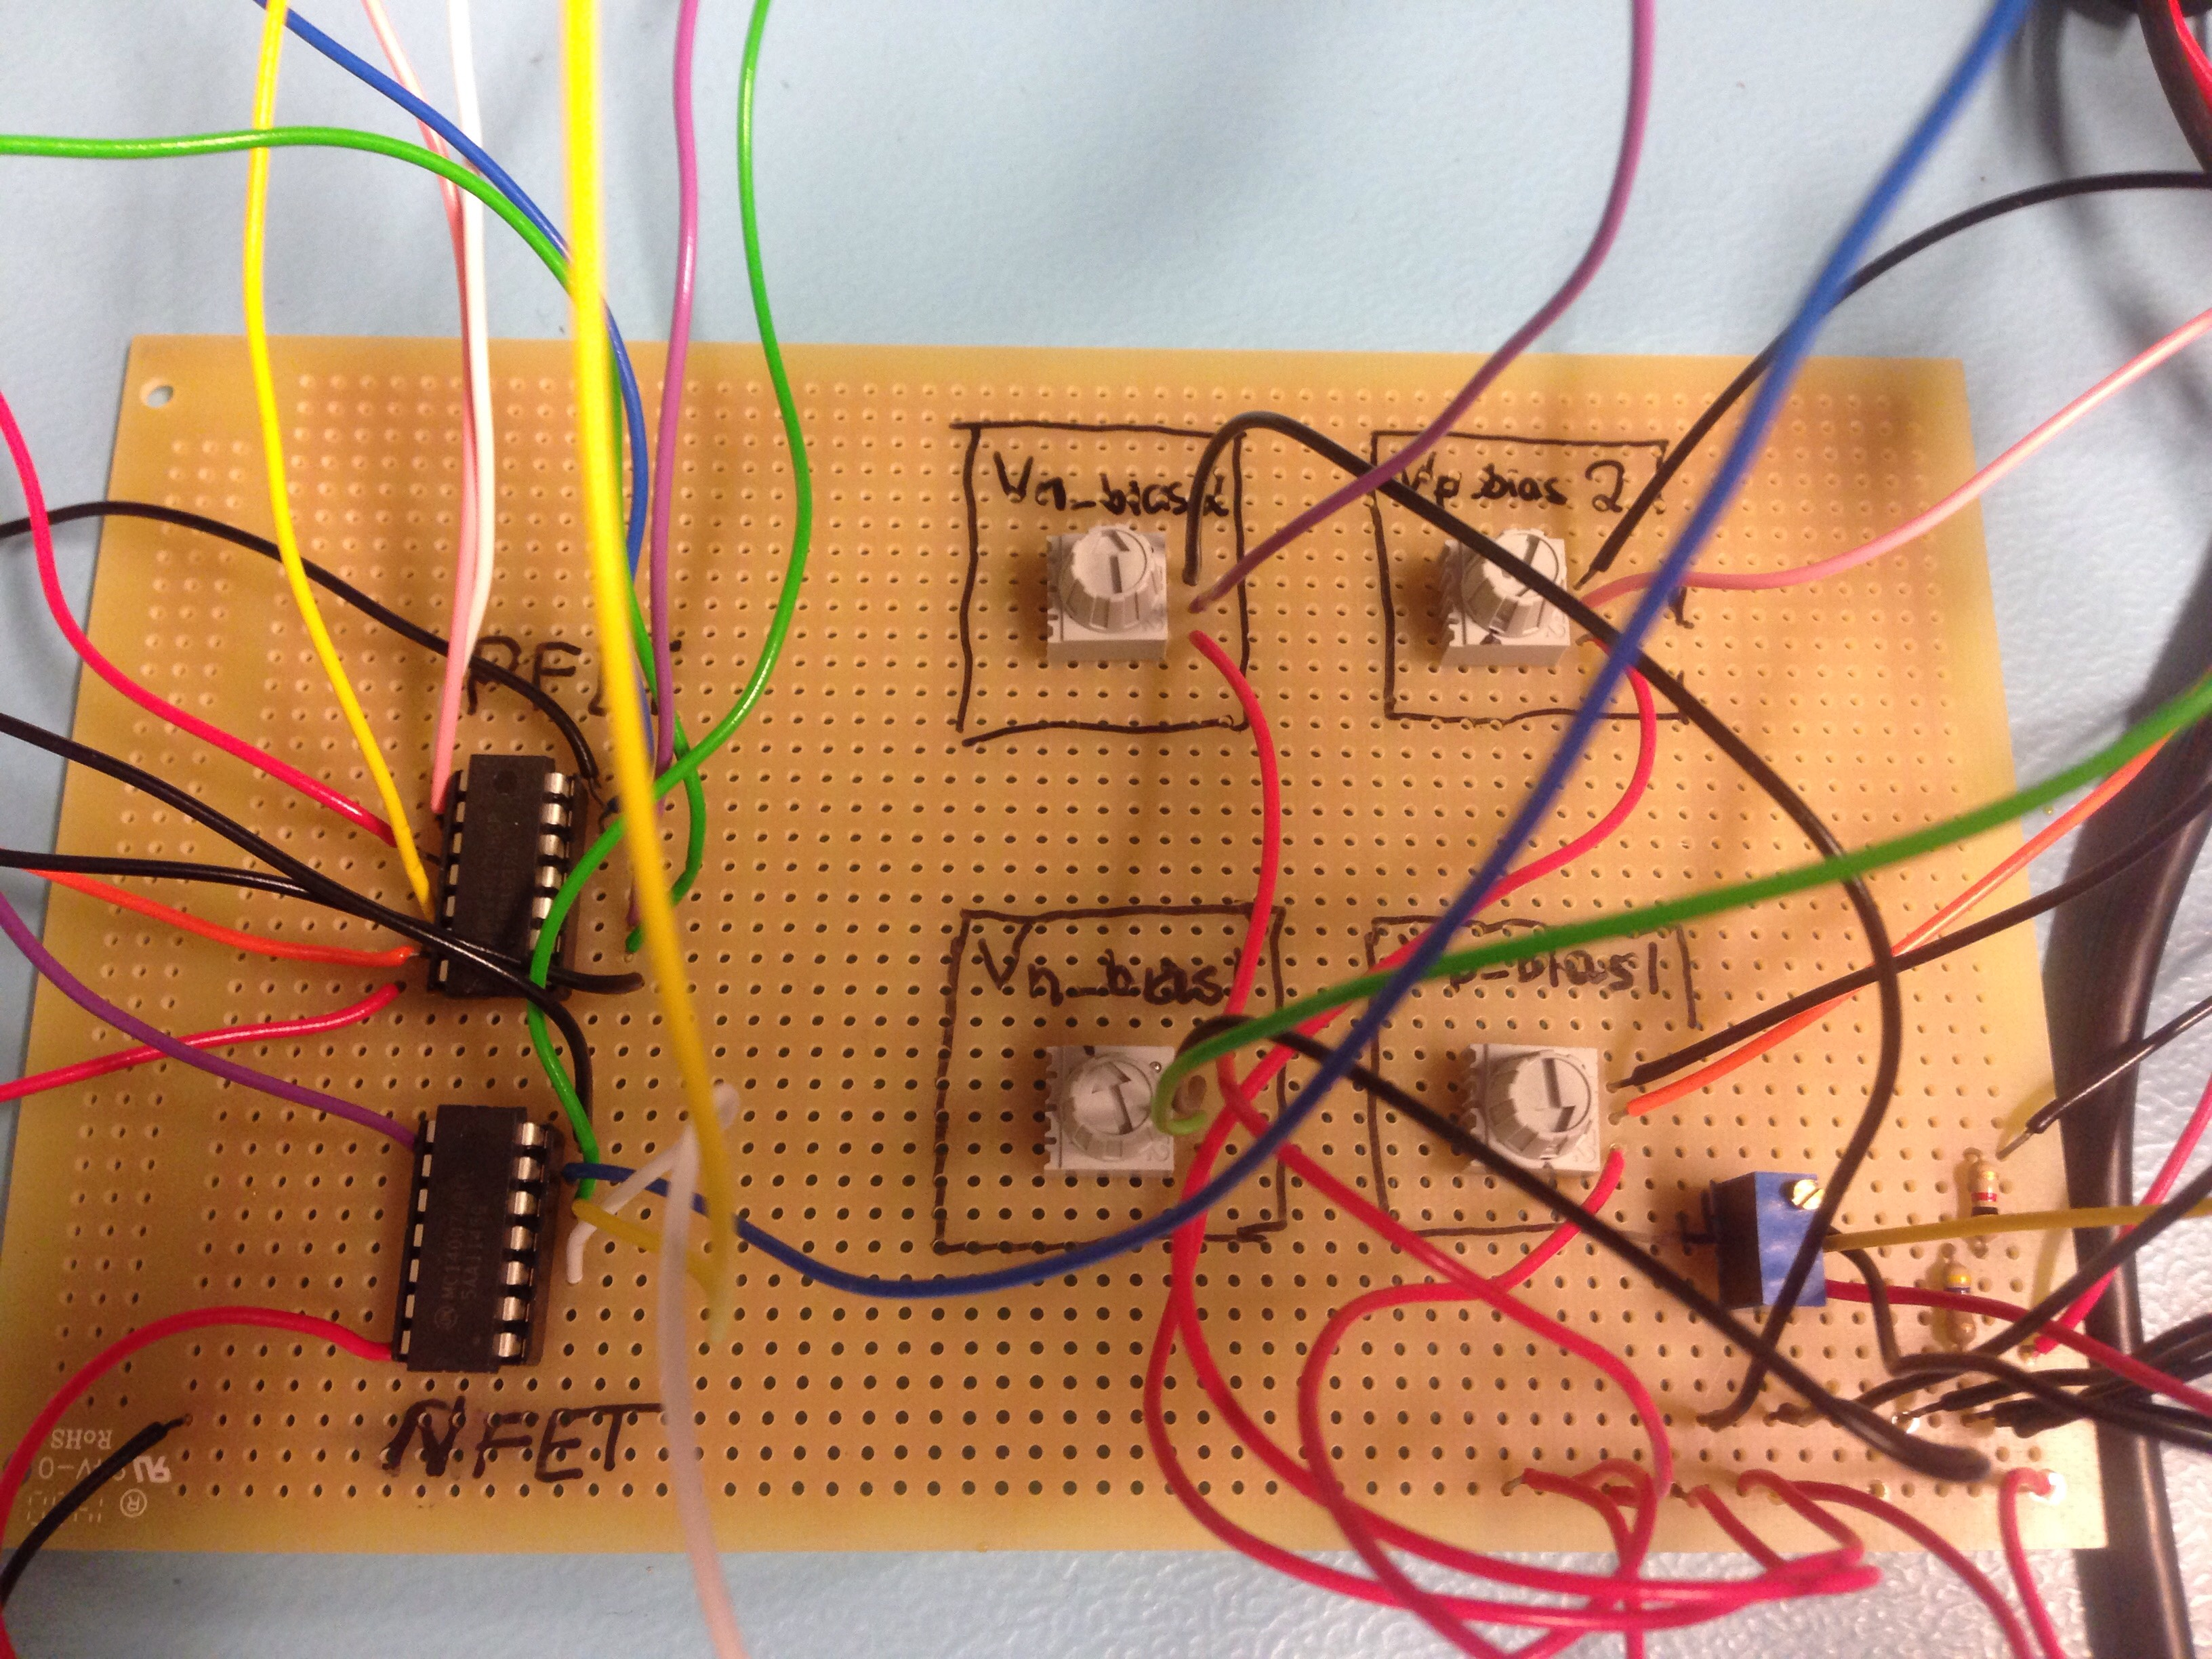
\includegraphics[width=\textwidth]{img/pcb_setup}}
%  \caption{Final PCB board.}
%  \label{fig:pcb}	
%s\end{figure}



\end{document}
